\section{ХОД РАБОТЫ}

\subsection{Постановка задачи}

Необходимо написать пару функций на языке Ассемблер,
которая бы осуществляла конвертацию температуры, выраженной в градусах 
Цельсия, в градусы Фаренгейта, и обратно.
Конвертация температуры должна производиться с использованием команд сопроцессора.

На языке высокого уровня необходимо осуществить вызов данных функций с
целью построения графика зависимости температуры, выраженной в градусах
различных шкал.

\subsection{Особенности разработанной программы}

Функция перевода температуры, выраженной в градусах Цельсия, в градусы Фаренгейта,
представлена на рисунке~\ref{lst:asm_c_f}.

\begin{lstlisting}[caption=Функция перевода температуры,
label=lst:asm_c_f,language={[x86masm]Assembler},basicstyle=\scriptsize\ttfamily]
 default rel                     ; relative address mode
 global  c_f:function
     
 segment .data
     input       dq 0
     output      dq 0
     nine        dq 9.e0
     five        dq 5.e0
     thirty_two  dq 32.e0
 
 segment .text
 c_f:
     push        rbp
     mov         rbp, rsp
 
     movlps      [input], xmm0
     
     finit
 
     fld        qword  [input]
     fmul       qword  [nine]
     fdiv       qword  [five]
     fadd       qword  [thirty_two]
     fstp       qword  [output]
                        
     movlps     xmm0,  [output]
     
     mov        rsp, rbp
     pop        rbp
     ret
\end{lstlisting}

Следует отметить, что использование сопроцессора для обработки данных 
позволяет существенно сократить объем кода. Директива default rel предписывает
использование адресации значений, расположенных в оперативной памяти,
относительно текущего значения RIP. Этот подход позволяет производить обращение
к данным независимо от адреса глобальной таблицы адресации GOT, которую
обычно приходится учитывать при создании динамических библиотек.

Директива global объявляет функцию c\_f видимой для других объектных модулей. 

Команда movlps используется для пересылки 64-битных данных между памятью и 
младшими 64-мя битами регистра xmm.

Основной интерес представляет собой построение графика зависимости
значений температурных шкал.
Дело в том, что в языке С нет достаточно простых
средств построения и вывода графиков такого рода.
С другой стороны, существует достаточно мощный пакет,
предназначенный для визуализации математических моделей,
написанный на языке Python, под названием matplotlib. 
Кроме этого, существует возможность создавать собственные модули Python,
используя язык программирования C.

Таким образом, написанную функцию перевода температуры можно обернуть
в специальным образом оформленный код на языке C, который можно использовать
как модуль Python. Средствами библиотеки matplotlib произвести вывод графика на экран,
а также в файл в виде изображения.

Рассмотрим код-обертку функции перевода температуры, приведенную на рисунке~\ref{lst:c_wrapper}.

В первой строке происходит включение header-файла Python.h, в котором
содержатся макросы для обеспечения совместимости типов языков C и Python.
Дело в том, что Python не является строго типизированным языком, 
в отличие от С, поэтому для создания объектов, видимых в среде Python, 
неоходимо использовать специальные функции, объявленные в этом файле.

Строка, начинающаеся с extern\dots, предназначена для связывания
функции ковертации температуры, написанной на языке Ассемблер,
с функцией c\_f языка С.

\pagebreak

\begin{lstlisting}[caption=Функция-обертка перевода температуры,
label=lst:c_wrapper,language={C},basicstyle=\scriptsize\ttfamily]
 #include <python2.7/Python.h>

 extern double c_f(double c);

 static PyObject *  py_ext_c2f(PyObject *self, PyObject *args) {
   double c;   
   if (!PyArg_ParseTuple(args, "d", &c))
     return NULL;
   return Py_BuildValue("d", c_f(c));
 }
 
 static PyMethodDef ModuleMethods[] = {
   { "c2f", py_ext_c2f, METH_VARARGS, "Convert Celsius to Fahrengheit" },
   {NULL, NULL, 0, NULL}
 };
 
 PyMODINIT_FUNC inittemperature(void) {
   Py_InitModule("temperature", ModuleMethods);
 }
\end{lstlisting}

Функция py\_ext\_c2f выполняет следующие действия:

\begin{enumerate}
\item конвертирует объект Python (args) в значение типа double языка C;
\item вызывает функцию, написанную на языке Ассемблер, 
  передавая ему в качестве аргумента значение типа double;
\item упаковывает возвращаемый аргумент в объект типа PyObject*. 
\end{enumerate}

Массив ModuleMethods содержит перечисление функций, которые будут видимы 
в модуле Python. 
Вызов функции Py\_InitModule с указанием данного перечисления выполняет регистрацию
этих функций в модуле Python.

После этого необходимо выполнить сборку модуля Python. 
Сначала необходимо скомпилировать код на языке Ассемблер, использую компилятор с
поддержкой платформы x86\_64, а затем собрать динамическую библиотеку для
обеспечения связывания с Python.
К счастью, для этой цели можно использовать пакет distutils, который
существенно упрощает процесс построения и инсталляции модуля.

Создадим файл setup.py, приведенный на рисунке~\ref{lst:setup_py}.

В этом файле указаны следующие параметры:
\begin{itemize}
\item название модуля;
\item версия;
\item описание модуля;
\item исходный код расширения, написанного на языке C;
\item дополнительные аргументы, передаваемые линковщику.
\end{itemize}

\begin{lstlisting}[caption=Параметры создания модуля Python,
label=lst:setup_py,language={Python},basicstyle=\scriptsize\ttfamily]
 from distutils.core import setup, Extension 
 setup(
     name = "Temperature",
     version = "0.0.0.1",
     description = "Temperature convertion functions",
     ext_modules = [Extension("temperature",
                              sources = ['temperature/tmp_module.c'],
                              # link with asm lib
                              extra_link_args = ['temperature/asm/tmp.o']),],
 )
\end{lstlisting}

Нетрудно догадаться, что в качестве дополнительно параметра, 
передаваемого линковщику, передается объектный файл, полученный
в результате компиляции кода функций конвертации температуры.

Сборка модуля python осуществляется с помощью команд,
приведенных на рисунке~\ref{lst:build_commands}.

\begin{lstlisting}[caption=Команды создания модуля Python,
label=lst:build_commands,language={bash},basicstyle=\scriptsize\ttfamily]
 nasm -g -f elf64 -o tmp.o tmp.asm
 python setup.py install
\end{lstlisting}

Наконец, создадим файл plot.py с исходным кодом, выполняющим построение требуемого 
графика, как показано на рисунке~\ref{lst:plot_py}.

\begin{lstlisting}[caption=Исходный код построения графика завимости температуры,
label=lst:plot_py,language={Python},basicstyle=\scriptsize\ttfamily]
 import matplotlib.pyplot as plt
 import temperature as tmp

 c = [x / 0.8 for x in range(-100, 100, 5)]
 f = map(tmp.c2f, c)

 plt.xlabel("Celsius")
 plt.ylabel("Fahrenheight")
 plt.grid(True)
 plt.plot(c, f,
          color="b", linestyle="--",
          marker=".", markersize=10, mfc="r")
 plt.show()
\end{lstlisting}

Данный код вычисляет ряд температур, выраженных в градусах Фаренгейта, соответствующий
ряду $ [-125; 125] $ в градусах Цельсия, графика с предварительной настройкой 
стиля отображения.

Результат работы программы приведен на рисунке~\ref{pic:result}.

\begin{figure}[h!]
  \centering
  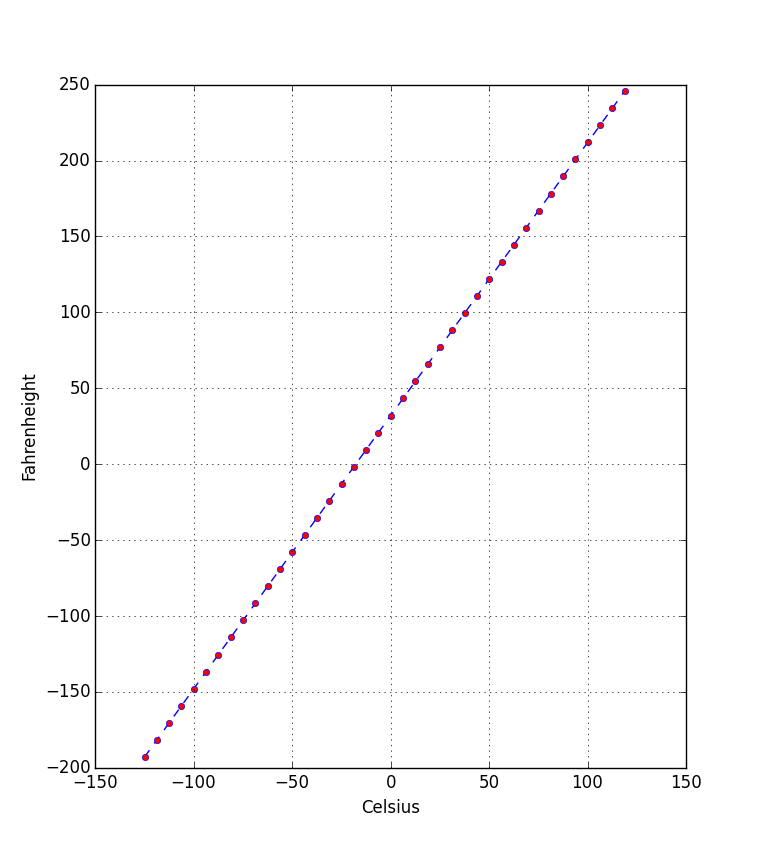
\includegraphics[width=0.8\linewidth]{pic/result}
  \caption{Результат работы программы}
  \label{pic:result}
\end{figure}

Исходный текст разработанной программы находится в приложении~А.
